\subsection{Our Parallel Naive-dynamic (ND) Leiden}
\label{sec:our-naive}

Algorithm \ref{alg:naive} details our multicore implementation of Naive dynamic (ND) Leiden. Here, vertices are assigned to communities based on the previous snapshot of the graph, with all vertices being processed regardless of edge deletions and insertions in the batch update. The algorithm accepts the current/updated graph snapshot $G^t$, edge deletions $\Delta^{t-}$ and insertions $\Delta^{t+}$ in the batch update, the previous community membership $C^{t-1}$ for each vertex, the weighted degree of each vertex $K^{t-1}$, and the total edge weight of each community $\Sigma^{t-1}$. The output includes the updated community memberships $C^t$, the updated weighted degrees $K^t$, and the updated total edge weights of communities $\Sigma^t$.

In the algorithm, we begin by defining two lambda functions for the Leiden algorithm: \texttt{isAffected()} (lines \ref{alg:naive--isaff-begin} to \ref{alg:naive--isaff-end}) and \texttt{inAffected} \texttt{Range()} (lines \ref{alg:naive--isaffrng-begin} to \ref{alg:naive--isaffrng-end}). These functions indicate that all vertices in the graph $G^t$ should be marked as affected and that these vertices can be incrementally marked as affected, respectively. Unlike previous approaches, we then use $K^{t-1}$ and $\Sigma^{t-1}$, along with the batch updates $\Delta^{t-}$ and $\Delta^{t+}$, to quickly compute $K^t$ and $\Sigma^t$, which are required for the local-moving phase of the Leiden algorithm (line \ref{alg:naive--auxliliary}). The lambda functions, along with the total vertex and edge weights, are then employed to run the Leiden algorithm and obtain\ignore{the} updated community assignments $C^t$ (line \ref{alg:naive--leiden}). Finally, $C^t$ is returned, along with $K^t$ and $\Sigma^t$ as\ignore{the} updated auxiliary information (line \ref{alg:naive--return}).

\begin{algorithm}[hbtp]
\caption{Our Parallel \textit{Naive-dynamic (ND)} Leiden \cite{sahu2024dflouvain}.}
\label{alg:naive}
\begin{algorithmic}[1]
\Require{$G^t(V^t, E^t)$: Current/updated input graph}
\Require{$\Delta^{t-}, \Delta^{t+}$: Edge deletions and insertions (batch update)}
\Require{$C^{t-1}, C^t$: Previous, current community of each vertex}
\Require{$K^{t-1}, K^t$: Previous, current weighted-degree of vertices}
\Require{$\Sigma^{t-1}, \Sigma^t$: Previous, current total edge weight of communities}
\Ensure{$isAffected(i)$: Is vertex $i$ is marked as affected?}
\Ensure{$inAffectedRange(i)$: Can $i$ be incrementally marked?}
\Ensure{$F$: Lambda functions passed to parallel Leiden (Alg. \ref{alg:leiden})}

\Statex

\Function{naiveDynamic}{$G^t, \Delta^{t-}, \Delta^{t+}, C^{t-1}, K^{t-1}, \Sigma^{t-1}$}
  \State $\rhd$ Mark affected vertices
  \Function{isAffected}{$i$} \label{alg:naive--isaff-begin}
    \Return{$1$}
  \EndFunction \label{alg:naive--isaff-end}
  \Function{inAffectedRange}{$i$} \label{alg:naive--isaffrng-begin}
    \Return{$1$}
  \EndFunction \label{alg:naive--isaffrng-end}
  \State $F \gets \{isAffected, inAffectedRange\}$ \label{alg:naive--lambdas}
  \State $\rhd$ Use $K^{t-1}$, $\Sigma^{t-1}$ as auxiliary information (Alg. \ref{alg:update})
  \State $\{K^t, \Sigma^t\} \gets updateWeights(G^t, \Delta^{t-}, \Delta^{t+}, C^{t-1}, K^{t-1}, \Sigma^{t-1})$\label{alg:naive--auxliliary}
  \State $\rhd$ Obtain updated communities (Alg. \ref{alg:leiden})
  \State $C^t \gets leiden(G^t, C^{t-1}, K^t, \Sigma^t, F)$ \label{alg:naive--leiden}
  \Return{$\{C^t, K^t, \Sigma^t\}$} \label{alg:naive--return}
\EndFunction
\end{algorithmic}
\end{algorithm}

\begin{algorithm}[hbtp]
\caption{Our Parallel \textit{Delta-screening (DS)} Leiden \cite{sahu2024dflouvain}.}
\label{alg:delta}
\begin{algorithmic}[1]
\Require{$G^t(V^t, E^t)$: Current/updated input graph}
\Require{$\Delta^{t-}, \Delta^{t+}$: Edge deletions and insertions (batch update)}
\Require{$C^{t-1}, C^t$: Previous, current community of each vertex}
\Require{$K^{t-1}, K^t$: Previous, current weighted-degree of vertices}
\Require{$\Sigma^{t-1}, \Sigma^t$: Previous, current total edge weight of communities}
\Ensure{$\delta V, \delta E, \delta C$: Is vertex, neighbors, or community affected?}
\Ensure{$H$: Hashtable mapping a community to associated weight}
\Ensure{$isAffected(i)$: Is vertex $i$ is marked as affected?}
\Ensure{$inAffectedRange(i)$: Can $i$ be incrementally marked?}
\Ensure{$F$: Lambda functions passed to parallel Leiden (Alg. \ref{alg:leiden})}

\Statex

\Function{deltaScreening}{$G^t, \Delta^{t-}, \Delta^{t+}, C^{t-1}, K^{t-1}, \Sigma^{t-1}$}
  \State $H, \delta V, \delta E, \delta C \gets \{\}$ \label{alg:delta--init}
  \State $\rhd$ Mark affected vertices
  \ForAll{$(i, j, w) \in \Delta^{t-}$ \textbf{in parallel}} \label{alg:delta--loopdel-begin}
    \If{$C^{t-1}[i] = C^{t-1}[j]$}
      \State $\delta V[i], \delta E[i], \delta C[C^{t-1}[j]] \gets 1$ \label{alg:delta--loopdelmark}
    \EndIf
  \EndFor \label{alg:delta--loopdel-end}
  \ForAll{unique source vertex $i \in \Delta^{t+}$ \textbf{in parallel}} \label{alg:delta--loopins-begin}
    \State $H \gets \{\}$
    \ForAll{$(i', j, w) \in \Delta^{t+}\ |\ i' = i$} \label{alg:delta--loopinssrc-begin}
      \If{$C^{t-1}[i] \neq C^{t-1}[j]$}
        \State $H[C^{t-1}[j]] \gets H[C^{t-1}[j]] + w$
      \EndIf
    \EndFor \label{alg:delta--loopinssrc-end}
    \State $c^* \gets$ Best community linked to $i$ in $H$ \label{alg:delta--loopinschoose}
    \State $\delta V[i], \delta E[i], \delta C[c^*] \gets 1$ \label{alg:delta--loopinsmark}
  \EndFor \label{alg:delta--loopins-end}
  \ForAll{$i \in V^t$ \textbf{in parallel}} \label{alg:delta--loopaff-begin}
    \If{$\delta E[i]$} \label{alg:delta--loopaffnei-begin}
      \ForAll{$j \in G^t.neighbors(i)$}
        \State $\delta V[j] \gets 1$
      \EndFor
    \EndIf \label{alg:delta--loopaffnei-end}
    \If{$\delta C[C^{t-1}[i]]$} \label{alg:delta--loopaffcom-begin}
      \State $\delta V[i] \gets 1$
    \EndIf \label{alg:delta--loopaffcom-end}
  \EndFor \label{alg:delta--loopaff-end}
  \Function{isAffected}{$i$} \label{alg:delta--isaff-begin}
    \Return{$\delta V[i]$}
  \EndFunction \label{alg:delta--isaff-end}
  \Function{inAffectedRange}{$i$} \label{alg:delta--isaffrng-begin}
    \Return{$\delta V[i]$}
  \EndFunction \label{alg:delta--isaffrng-end}
  \State $F \gets \{isAffected, inAffectedRange\}$ \label{alg:delta--lambdas}
  \State $\rhd$ Use $K^{t-1}$, $\Sigma^{t-1}$ as auxiliary information (Alg. \ref{alg:update})
  \State $\{K^t, \Sigma^t\} \gets updateWeights(G^t, \Delta^{t-}, \Delta^{t+}, C^{t-1}, K^{t-1}, \Sigma^{t-1})$\label{alg:delta--auxiliary}
  \State $\rhd$ Obtain updated communities (Alg. \ref{alg:leiden})
  \State $C^t \gets leiden(G^t, C^{t-1}, K^t, \Sigma^t, F)$ \label{alg:delta--leiden}
  \Return{$\{C^t, K^t, \Sigma^t\}$} \label{alg:delta--return}
\EndFunction
\end{algorithmic}
\end{algorithm}





\subsection{Our Parallel Delta-screening (DS) Leiden}
\label{sec:our-delta}

Algorithm \ref{alg:delta} presents the pseudocode for our multicore implementation of Delta-screening (DS) Leiden. It employs modularity-based scoring to identify an approximate region of the graph where vertices are likely to change their community membership \cite{com-zarayeneh21}. It takes as input the current/updated graph snapshot $G^t$, edge deletions $\Delta^{t-}$ and insertions $\Delta^{t+}$ in the batch update, the previous community memberships of vertices $C^{t-1}$, the weighted degrees of vertices $K^{t-1}$, and the total edge weights of communities $\Sigma^{t-1}$. The algorithm outputs the updated community memberships $C^t$, weighted degrees $K^t$, and total edge weights of communities $\Sigma^t$. Prior to processing, the batch update --- which includes edge deletions $(i, j, w) \in \Delta^{t-}$ and insertions $(i, j, w) \in \Delta^{t+}$ --- are sorted separately by the source vertex ID $i$.

In the algorithm, we start by initializing a hashtable $H$ that maps communities to their associated weights, and we set the affected flags $\delta V$, $\delta E$, and $\delta C$, which indicate whether a vertex, its neighbors, or its community is affected by the batch update (lines \ref{alg:delta--init}). We then parallelly process edge deletions $\Delta^{t-}$ and insertions $\Delta^{t+}$. For each deletion $(i, j, w) \in \Delta^{t-}$ where vertices $i$ and $j$ belong to the same community, we mark the source vertex $i$, its neighbors, and its community as affected (lines \ref{alg:delta--loopdel-begin}-\ref{alg:delta--loopdel-end}). For each unique source vertex $i$ in insertions $(i, j, w) \in \Delta^{t+}$ where $i$ and $j$ belong to different communities, we determine the community $c^*$ with the highest delta-modularity if $i$ moves to one of its neighboring communities, marking $i$, its neighbors, and the community $c^*$ as affected (lines \ref{alg:delta--loopins-begin}-\ref{alg:delta--loopins-end}). We disregard deletions between different communities and insertions within the same community. Using the affected neighbor $\delta E$ and community flags $\delta C$, we mark affected vertices in $\delta V$ (lines \ref{alg:delta--loopaff-begin}-\ref{alg:delta--loopaff-end}). Subsequently, similar to ND Leiden, we utilize $K^{t-1}$ and $\Sigma^{t-1}$, along with $\Delta^{t-}$ and $\Delta^{t+}$, to quickly derive $K^t$ and $\Sigma^t$ (line \ref{alg:naive--auxliliary}). We define the necessary lambda functions \texttt{isAffected()} (lines \ref{alg:delta--isaff-begin}-\ref{alg:delta--isaff-end}) and \texttt{inAffectedRange()} (lines \ref{alg:delta--isaffrng-begin}-\ref{alg:delta--isaffrng-end}), and execute the Leiden algorithm, resulting in updated community assignments $C^t$ (line \ref{alg:delta--leiden}). Finally, we return\ignore{the} updated community memberships $C^t$ along with $K^t$ and $\Sigma^t$ as\ignore{the} updated auxiliary information (line \ref{alg:delta--return}).




\subsection{Our Parallel Dynamic Frontier (DF) Leiden}
\label{sec:our-frontier}

Algorithm \ref{alg:frontier} presents the pseudocode for our Parallel Dynamic Frontier (DF) Leiden. It takes as input the updated graph snapshot $G^t$, edge deletions $\Delta^{t-}$ and insertions $\Delta^{t+}$ from the batch update, the previous community assignments $C^{t-1}$ for each vertex, the previous weighted degrees $K^{t-1}$ of vertices, and the previous total edge weights $\Sigma^{t-1}$ of communities. It outputs the updated community memberships $C^t$ for vertices, the updated weighted degrees $K^t$ of vertices, and the updated total edge weights $\Sigma^t$ of communities.

\begin{algorithm}[hbtp]
\caption{Our Parallel \textit{Dynamic Frontier (DF)} Leiden \cite{sahu2024dflouvain}.}
\label{alg:frontier}
\begin{algorithmic}[1]
\Require{$G^t(V^t, E^t)$: Current/updated input graph}
\Require{$\Delta^{t-}, \Delta^{t+}$: Edge deletions and insertions (batch update)}
\Require{$C^{t-1}, C^t$: Previous, current community of each vertex}
\Require{$K^{t-1}, K^t$: Previous, current weighted-degree of vertices}
\Require{$\Sigma^{t-1}, \Sigma^t$: Previous, current total edge weight of communities}
\Ensure{$\delta V$: Flag vector indicating if each vertex is affected}
\Ensure{$isAffected(i)$: Is vertex $i$ is marked as affected?}
\Ensure{$inAffectedRange(i)$: Can $i$ be incrementally marked?}
\Ensure{$onChange(i)$: What happens if $i$ changes its community?}
\Ensure{$F$: Lambda functions passed to parallel Leiden (Alg. \ref{alg:leiden})}

\Statex

\Function{dynamicFrontier}{$G^t, \Delta^{t-}, \Delta^{t+}, C^{t-1}, K^{t-1}, \Sigma^{t-1}$}
  \State $\rhd$ Mark initial affected vertices
  \ForAll{$(i, j) \in \Delta^{t-}$ \textbf{in parallel}} \label{alg:frontier--loopdel-begin}
    \If{$C^{t-1}[i] = C^{t-1}[j]$} $\delta V[i] \gets 1$
    \EndIf
  \EndFor \label{alg:frontier--loopdel-end}
  \ForAll{$(i, j, w) \in \Delta^{t+}$ \textbf{in parallel}} \label{alg:frontier--loopins-begin}
    \If{$C^{t-1}[i] \neq C^{t-1}[j]$} $\delta V[i] \gets 1$
    \EndIf
  \EndFor \label{alg:frontier--loopins-end}
  \Function{isAffected}{$i$} \label{alg:frontier--isaff-begin}
    \Return{$\delta V[i]$}
  \EndFunction \label{alg:frontier--isaff-end}
  \Function{inAffectedRange}{$i$} \label{alg:frontier--isaffrng-begin}
    \Return{$1$}
  \EndFunction \label{alg:frontier--isaffrng-end}
  \Function{onChange}{$i$} \label{alg:frontier--onchg-begin}
    \ForAll{$j \in G^t.neighbors(i)$} $\delta V[j] \gets 1$
    \EndFor
  \EndFunction \label{alg:frontier--onchg-end}
  \State $F \gets \{isAffected, inAffectedRange, onChange\}$ \label{alg:frontier--lambdas}
  \State $\rhd$ Use $K^{t-1}$, $\Sigma^{t-1}$ as auxiliary information (Alg. \ref{alg:update})
  \State $\{K^t, \Sigma^t\} \gets updateWeights(G^t, \Delta^{t-}, \Delta^{t+}, C^{t-1}, K^{t-1}, \Sigma^{t-1})$\label{alg:frontier--auxiliary}
  \State $\rhd$ Obtain updated communities (Alg. \ref{alg:leiden})
  \State $C^t \gets leiden(G^t, C^{t-1}, K^t, \Sigma^t, F)$ \label{alg:frontier--leiden}
  \Return{$\{C^t, K^t, \Sigma^t\}$} \label{alg:frontier--return}
\EndFunction
\end{algorithmic}
\end{algorithm}


In the algorithm, we initially identify a set of affected vertices whose communities may directly change due to batch updates by marking them in the flag vector $\delta V$. This is achieved by marking the endpoints of edge deletions $\Delta^{t-}$ that lie within the same community (lines \ref{alg:frontier--loopdel-begin}-\ref{alg:frontier--loopdel-end}), and by marking the endpoints of edge insertions $\Delta^{t+}$ that lie in disjoint communities (lines \ref{alg:frontier--loopins-begin}-\ref{alg:frontier--loopins-end}). Subsequently, three lambda functions are defined for the Leiden algorithm: \texttt{isAffected()} (lines \ref{alg:frontier--isaff-begin}-\ref{alg:frontier--isaff-end}), \texttt{inAffectedRange()} (lines \ref{alg:frontier--isaffrng-begin}-\ref{alg:frontier--isaffrng-end}), and \texttt{onChange()} (lines \ref{alg:frontier--onchg-begin}-\ref{alg:frontier--onchg-end}). These functions indicate that a set of vertices are initially marked as affected, that all vertices in the graph can be incrementally marked as affected, and that the neighbors of a vertex are marked as affected if it changes its community membership, respectively. It is important to note that the set of affected vertices will expand automatically due to vertex pruning optimization used in our Parallel Leiden algorithm (Algorithm \ref{alg:leiden}). Thus, \texttt{onChange()} reflects what the DF approach would do in the absence of vertex pruning. Additionally, unlike existing approaches, we utilize $K^{t-1}$ and $\Sigma^{t-1}$, alongside the batch updates $\Delta^{t-}$ and $\Delta^{t+}$, to efficiently compute $K^t$ and $\Sigma^t$ required for the local-moving phase of the Leiden algorithm (line \ref{alg:frontier--auxiliary}). These lambda functions and the total vertex/edge weights are then employed to execute the Leiden algorithm and obtain the updated community assignments $C^t$ (line \ref{alg:frontier--leiden}). Finally, we return $C^t$, alongside $K^t$ and $\Sigma^t$\ignore{, serving as the updated auxiliary information} (line \ref{alg:frontier--return}).




\subsection{Our Dynamic-supporting Parallel Leiden}
\label{sec:our-leiden}

The main step of our Dynamic-supporting Parallel Leiden is outlined in Algorithm \ref{alg:leiden}. In contrast to our implementation of Static Leiden \cite{sahu2023gveleiden}, this algorithm, in addition to the current graph snapshot $G^t$, accepts the prior community membership of each vertex $C^{t-1}$, the revised weighted degree of each vertex $K^t$, the updated total edge weight of each community $\Sigma^t$, and a set of lambda functions $F$ determining whether a vertex is influenced or can be progressively identified as influenced (within the affected range). It yields the updated community memberships of vertices $C^t$.

\begin{algorithm}[hbtp]
\caption{Our Dynamic-supporting Parallel Leiden \cite{sahu2023gveleiden}.}
\label{alg:leiden}
\begin{algorithmic}[1]
\Require{$G^t$: Current input graph}
\Require{$C^{t-1}$: Previous community of each vertex}
\Require{$K^t$: Current weighted-degree of each vertex}
\Require{$\Sigma^t$: Current total edge weight of each community}
\Require{$F$: Lambda functions passed to parallel Leiden}
\Ensure{$G'$: Current/super-vertex graph.}
\Ensure{$C, C'$: Current community of each vertex in $G^t$, $G'$}
\Ensure{$K, K'$: Current weighted-degree of each vertex in $G^t$, $G'$}
\Ensure{$\Sigma, \Sigma'$: Current total edge weight of each community in $G^t$, $G'$}
\Ensure{$\tau, \tau_{agg}$: Iteration, aggregation tolerance}

\Statex

\Function{leiden}{$G^t, C^{t-1}, K^t, \Sigma^t, F$} \label{alg:leiden--begin}
  \State $\rhd$ Mark affected vertices as unprocessed
  \ForAll{$i \in V^t$} \label{alg:leiden--mark-begin}
    \If{$F.isAffected(i)$} Mark $i$ as unprocessed
    \EndIf
  \EndFor \label{alg:leiden--mark-end}
  \State $\rhd$ Initialization phase
  \State Vertex membership: $C \gets [0 .. |V^t|)$ \label{alg:leiden--init-begin}
  \State $G' \gets G^t$ \textbf{;} $C' \gets C^{t-1}$ \textbf{;} $K' \gets K^t$ \textbf{;} $\Sigma' \gets \Sigma^t$ \label{alg:leiden--init-end}
  \State $\rhd$ Local-moving and aggregation phases
  \ForAll{$l_p \in [0 .. \text{\small{MAX\_PASSES}})$} \label{alg:leiden--passes-begin}
    \State $l_i \gets leidenMove(G', C', K', \Sigma', F)$ \Comment{Alg. \ref{alg:leidenlm}} \label{alg:leiden--local-move}
    \State $C'_B \gets C'$ \textbf{;} $C' \gets [0 .. |V'|)$ \textbf{;} $\Sigma' \gets K'$ \label{alg:leiden--reset-again}
    \State $l_j \gets leidenRefine(G', C'_B, C', K', \Sigma', \tau)$ \Comment{Alg. \ref{alg:leidenre}} \label{alg:leiden--refine}
    \If{\textbf{not} first pass \textbf{and} $l_i + l_j \le 1$} \textbf{break} \Comment{Done?} \label{alg:leiden--globally-converged}
    \EndIf
    \State $|\Gamma|, |\Gamma_{old}| \gets$ Number of communities in $C$, $C'$
    \If{$|\Gamma|/|\Gamma_{old}| > \tau_{agg}$} \textbf{break} \Comment{Low shrink?} \label{alg:leiden--aggregation-tolerance}
    \EndIf
    \State $C' \gets$ Renumber communities in $C'$ \label{alg:leiden--renumber}
    \State $C \gets$ Lookup dendrogram using $C$ to $C'$ \label{alg:leiden--lookup}
    \State $G' \gets leidenAggregate(G', C')$ \Comment{Alg. \ref{alg:leidenag}} \label{alg:leiden--aggregate}
    \State $\Sigma' \gets K' \gets$ Weight of each vertex in $G'$ \label{alg:leiden--reset-weights}
    \State Mark all vertices in $G'$ as unprocessed \label{alg:leiden--reset-affected}
    \State $C' \gets [0 .. |V'|)$ \Comment{Use refine-based membership} \label{alg:leiden--useparent}
    % \State $C' \gets$ Map $C'$ to $C'_B$ \Comment{Use move-based membership} \label{alg:leiden--useparent}
    \State $\tau \gets \tau / \text{\small{TOLERANCE\_DROP}}$ \Comment{Threshold scaling} \label{alg:leiden--threshold-scaling}
  \EndFor \label{alg:leiden--passes-end}
  \State $C \gets$ Lookup dendrogram using $C$ to $C'$ \label{alg:leiden--lookup-last}
  \Return{$C$} \label{alg:leiden--return}
\EndFunction \label{alg:leiden--end}
\end{algorithmic}
\end{algorithm}




%% Parameter setting
% $\tau \gets TOLERANCE\_INITIAL$
% TOLERANCE\_INITIAL = 0.01
% TOLERANCE\_DECLINE = 10
% MAX\_PASSES = 500


In the algorithm, we start by marking the affected vertices as unprocessed (lines \ref{alg:leiden--mark-begin}-\ref{alg:leiden--mark-end}). Next, during the initialization phase, several parameters are set: the community membership of each vertex $C$ in $G^t$, the total edge weight of each vertex $K'$, the total edge weight of each community $\Sigma'$, and the community membership $C'$ of each vertex in the current (super-vertex) graph $G'$. Additionally, an initial set of changed communities $\Delta C'$ is determined based on the batch update as described in Section \ref{sec:approach} (lines \ref{alg:leiden--init-begin}-\ref{alg:leiden--init-end}). Following initialization, a series of passes is carried out, limited by $MAX\_PASSES$, with each pass comprising local-moving, refinement, and aggregation phases (lines \ref{alg:leiden--passes-begin}-\ref{alg:leiden--passes-end}). In each pass, the Leiden algorithm’s local-moving phase (Algorithm \ref{alg:leidenlm}) is executed to optimize community assignments (line \ref{alg:leiden--local-move}). However, this phase may result in poorly connected or internally disconnected communities. Therefore, the communities must be refined. For selective refinement --- which enhances the algorithm's efficiency for small batch updates --- the community IDs are renumbered so that each community ID corresponds to one of its constituent vertices. Additionally, the total edge weights of communities and the flags for changed communities are updated accordingly (see Algorithm \ref{alg:leidensr}), and changed communities are broken up, isolating their constituent vertices into separate communities. The total weights of these communities are adjusted as needed. The refinement phase, executed by \texttt{leidenRefine()}, optimizes the community assignments for each vertex within its community boundaries $C'_B$ obtained from the local-moving phase (line \ref{alg:leiden--refine}). If the local-moving phase converges after a single iteration, indicating global convergence, the passes are halted (line \ref{alg:leiden--globally-converged}). If convergence is not achieved, the aggregation phase is performed. This involves renumbering the communities, updating top-level community memberships $C$ using dendrogram lookup, performing the aggregation process (Algorithm \ref{alg:leidenag}), and updating the weighted degrees of vertices $K'$ and total edge weights of communities $\Sigma'$ in the super-vertex graph. Following this, to prepare for the next pass of the algorithm, we mark all vertices in this graph as unprocessed, initialize community memberships based on the refinement phase, mark all communities as changed for the next pass, and adjust the convergence threshold $\tau$ by scaling it (line \ref{alg:leiden--threshold-scaling}). The next pass then begins (line \ref{alg:leiden--passes-begin}). After all passes, the top-level community memberships $C$ of each vertex in $G^t$ are updated one final time via dendrogram lookup before being returned (lines \ref{alg:leiden--lookup-last}-\ref{alg:leiden--return}).

We now discuss about two support functions \textsc{changedCommunities()} and \textsc{breakChangedCommunities()}. The function \textsc{changedCommunities()} takes as input the batch update, consisting of edge deletions $\Delta^{t-}$ and insertions $\Delta^{t+}$, and marks a community as changed if both the endpoints of edge deletions and insertions belong to the same community. However, this is only done for ND, DS, and DF Leiden --- all communities are considered to haved changed with Static Leiden. Finally, the function \textsc{breakChangedCommunities()} splits changed communities, as indicated with the changed communities flag $\Delta C'$, into vertices belonging to isolated communities.


\subsubsection{Local-moving phase of our Parallel Leiden}

The pseudocode for the local-moving phase\ignore{of our Parallel Leiden} is presented in Algorithm \ref{alg:leidenlm}. It iteratively moves vertices among communities in order to maximize modularity. Here, the \texttt{leidenMove()} function operates on the current graph $G'$, community membership $C'$, total edge weight of each vertex $K'$, total edge weight of each community $\Sigma'$, changed communities flag vector $\Delta C'$, and a set of lambda functions as inputs, yielding the number of iterations performed $l_i$.

\begin{algorithm}[hbtp]
\caption{Local-moving phase of our Parallel Leiden \cite{sahu2024dflouvain}.}
\label{alg:leidenlm}
\begin{algorithmic}[1]
\Require{$G'$: Input/super-vertex graph}
\Require{$C'$: Community membership of each vertex}
\Require{$K'$: Total edge weight of each vertex}
\Require{$\Sigma'$: Total edge weight of each community}
\Require{$F$: Lambda functions passed to parallel Leiden}
\Ensure{$H_t$: Collision-free per-thread hashtable}
\Ensure{$l_i$: Number of iterations performed}
\Ensure{$\tau$: Per iteration tolerance}

\Statex

\Function{leidenMove}{$G', C', K', \Sigma', F$} \label{alg:leidenlm--move-begin}
  \ForAll{$l_i \in [0 .. \text{\small{MAX\_ITERATIONS}})$} \label{alg:leidenlm--iterations-begin}
    \State Total delta-modularity per iteration: $\Delta Q \gets 0$ \label{alg:leidenlm--init-deltaq}
    \ForAll{unprocessed $i \in V'$ \textbf{in parallel}} \label{alg:leidenlm--loop-vertices-begin}
      \State Mark $i$ as processed (prune) \label{alg:leidenlm--prune}
      \If{\textbf{not} $F.inAffectedRange(i)$} \textbf{continue} \label{alg:leidenlm--affrng}
      \EndIf
      \State $H_t \gets scanCommunities(\{\}, G', C', i, false)$ \label{alg:leidenlm--scan}
      \State $\rhd$ Use $H_t, K', \Sigma'$ to choose best community
      \State $c^* \gets$ Best community linked to $i$ in $G'$ \label{alg:leidenlm--best-community-begin}
      \State $\delta Q^* \gets$ Delta-modularity of moving $i$ to $c^*$ \label{alg:leidenlm--best-community-end}
      \If{$c^* = C'[i]$} \textbf{continue} \label{alg:leidenlm--best-community-same}
      \EndIf
      \State $\Sigma'[C'[i]] -= K'[i]$ \textbf{;} $\Sigma'[c^*] += K'[i]$ \textbf{atomic} \label{alg:leidenlm--perform-move-begin}
      \State $C'[i] \gets c^*$ \textbf{;} $\Delta Q \gets \Delta Q + \delta Q^*$ \label{alg:leidenlm--perform-move-end}
      \State Mark neighbors of $i$ as unprocessed \label{alg:leidenlm--remark}
    \EndFor \label{alg:leidenlm--loop-vertices-end}
    \If{$\Delta Q \le \tau$} \textbf{break} \Comment{Locally converged?} \label{alg:leidenlm--locally-converged}
    \EndIf
  \EndFor \label{alg:leidenlm--iterations-end}
  \Return{$l_i$} \label{alg:leidenlm--return}
\EndFunction \label{alg:leidenlm--move-end}

\Statex

\Function{scanCommunities}{$H_t, G', C', i, self$}
  \ForAll{$(j, w) \in G'.edges(i)$}
    \If{$self$ \textbf{or} $i \neq j$} $H_t \gets H_t[C'[j]] + w$
    \EndIf
  \EndFor
  \Return{$H_t$}
\EndFunction
\end{algorithmic}
\end{algorithm}




%% Parameter setting
% $\tau \gets TOLERANCE\_INITIAL$
% TOLERANCE\_INITIAL = 0.01
% TOLERANCE\_DECLINE = 10
% MAX\_PASSES = 500


Lines \ref{alg:leidenlm--iterations-begin}-\ref{alg:leidenlm--iterations-end} encapsulate the primary loop of the local-moving phase. In line \ref{alg:leidenlm--init-deltaq}, we initialize the total delta-modularity per iteration $\Delta Q$. Subsequently, in lines \ref{alg:leidenlm--loop-vertices-begin}-\ref{alg:leidenlm--loop-vertices-end}, we concurrently iterate over unprocessed vertices. For each vertex $i$, we perform vertex pruning by marking $i$ as processed (line \ref{alg:leidenlm--prune}). Next, we verify if $i$ falls within the affected range (i.e., it is permitted to be incrementally marked as affected), and if not, we proceed to the next vertex (line \ref{alg:leidenlm--affrng}). For each unskipped vertex $i$, we scan communities connected to $i$ (line \ref{alg:leidenlm--scan}), excluding itself, ascertain the optimal community $c*$ to move $i$ to (line \ref{alg:leidenlm--best-community-begin}), compute the delta-modularity of moving $i$ to $c*$ (line \ref{alg:leidenlm--best-community-end}), update the community membership of $i$ (lines \ref{alg:leidenlm--perform-move-begin}-\ref{alg:leidenlm--perform-move-end}), and mark its neighbors as unprocessed (line \ref{alg:leidenlm--remark}) if a superior community is identified. It is worth noting that this practice of marking neighbors of $i$ as unprocessed, which is part of the vertex pruning optimization, also aligns with algorithm of DF Leiden --- which marks its neighbors as affected, when a vertex changes its community. Thus, vertex pruning facilitates incremental expansion of the set of affected vertices without requiring any extra code. Further, for ND, DS, and DF Leiden, we mark the source $c$ and target communities $c^*$ of the migrating vertex $i$ as changed. With Static Leiden, all communities are always refined. In line \ref{alg:leidenlm--locally-converged}, we examine whether the local-moving phase has achieved convergence (locally); if so, the loop is terminated (or if $MAX\_ITERATIONS$ is reached). Finally, in line \ref{alg:leidenlm--return}, we return the number of iterations performed\ignore{by the local-moving phase} $l_i$.


\subsubsection{Refinement phase of our Parallel Leiden}

\begin{algorithm}[hbtp]
\caption{Refinement phase of our Parallel Leiden \cite{sahu2023gveleiden}.}
\label{alg:leidenre}
\begin{algorithmic}[1]
\Require{$G'$: Input/super-vertex graph}
\Require{$C'$: Community membership of each vertex}
\Require{$K'$: Total edge weight of each vertex}
\Require{$\Sigma'$: Total edge weight of each community}
\Ensure{$G'_{C'}$: Community vertices (CSR)}
\Ensure{$H_t$: Collision-free per-thread hashtable}
\Ensure{$\tau$: Per iteration tolerance}

\Statex

\Function{leidenRefine}{$G', C'_B, C', K', \Sigma', \tau$} \label{alg:leidenre--move-begin}
  \ForAll{$i \in V'$ \textbf{in parallel}} \label{alg:leidenre--loop-vertices-begin}
    \State $c \gets C'[i]$
    \If{$\Sigma'[c] \neq K'[i]$} \textbf{continue} \label{alg:leidenre--check-isolated}
    \EndIf
    \State $H_t \gets scanBounded(\{\}, G', C'_B, C', i, false)$ \label{alg:leidenre--scan}
    \State $\rhd$ Use $H_t, K', \Sigma'$ to choose best community
    \State $c^* \gets$ Best community linked to $i$ in $G'$ within $C'_B$ \label{alg:leidenre--best-community-begin}
    \State $\delta Q^* \gets$ Delta-modularity of moving $i$ to $c^*$ \label{alg:leidenre--best-community-end}
    \If{$c^* = c$} \textbf{continue} \label{alg:leidenre--best-community-same}
    \EndIf
    \If{$atomicCAS(\Sigma'[c], K'[i], 0) = K'[i]$} \label{alg:leidenre--perform-move-begin}
      \State $\Sigma'[c^*] += K'[i]$ \textbf{atomically}
      \State $C'[i] \gets c^*$ \label{alg:leidenre--perform-move-end}
    \EndIf
  \EndFor \label{alg:leidenre--loop-vertices-end}
\EndFunction \label{alg:leidenre--move-end}

\Statex

\Function{scanBounded}{$H_t, G', C'_B, C', i, self$}
  \ForAll{$(j, w) \in G'.edges(i)$}
    \If{\textbf{not} $self$ \textbf{and} $i = j$} \textbf{continue}
    \EndIf
    \If{$C'_B[i] \neq C'_B[j]$} \textbf{continue}
    \EndIf
    \State $H_t[C'[j]] \gets H_t[C'[j]] + w$
  \EndFor
  \Return{$H_t$}
\EndFunction

\Statex

\Function{atomicCAS}{$pointer, old, new$}
  \State $\rhd$ Perform the following atomically
  \If{$pointer = old$} $pointer \gets new$ \textbf{;} \ReturnInline{$old$}
  \Else\ \ReturnInline{$pointer$}
  \EndIf
\EndFunction
\end{algorithmic}
\end{algorithm}


The pseudocode outlining the refinement phase of our Parallel Leiden is presented in Algorithm \ref{alg:leidenlm}. This phase closely resembles the local-moving phase but incorporates the community membership obtained for each vertex as a \textit{community bound}. In this phase, each vertex is required to select a community within its community bound to join, aiming to maximize modularity through iterative movements between communities, akin to the local-moving phase. At the onset of the refinement phase, the community membership of each vertex is reset so that each vertex initially forms its own community. The \texttt{leidenRefine()} function is employed, taking as input the current graph $G'$, the community bound of each vertex $C'_B$, the initial community membership $C'$ of each vertex, the total edge weight of each vertex $K'$, the initial total edge weight of each community $\Sigma'$, changed communities flag vector $\Delta C'$, and the current tolerance per iteration $\tau$, and returns the number of iterations executed $l_j$.

Lines \ref{alg:leidenre--loop-vertices-begin}-\ref{alg:leidenre--loop-vertices-end} embody the central aspect of the refinement phase. During this phase, we execute what is termed the constrained merge procedure \cite{com-traag19}. The essence of this procedure lies in enabling vertices, within each community boundary, to create sub-communities solely by permitting isolated vertices (i.e., vertices belonging to their own community) to alter their community affiliation. This process divides any internally-disconnected communities identified during the local-moving phase and prevents the emergence of new disconnected communities. Specifically, for every isolated vertex $i$ (line \ref{alg:leidenre--check-isolated}), we explore communities connected to $i$ within the \textit{same community boundary} - excluding itself (line \ref{alg:leidenre--scan}). The refinement phase is skipped for a vertex if its community has not been flagged as changed ($\Delta C'[c] = 0$), or if another vertex has joined its community, as indicated by the total community weight no longer matching the total edge weight of the vertex. Subsequently, we determine the optimal community $c*$ for relocating $i$ (line \ref{alg:leidenre--best-community-begin}), and assess the delta-modularity of transferring $i$ to $c*$ (line \ref{alg:leidenre--best-community-end}). If a superior community is identified, we attempt to update the community affiliation of $i$ provided it remains isolated (lines \ref{alg:leidenre--perform-move-begin}-\ref{alg:leidenre--perform-move-end}). Note that we do not migrate the vertex $i$ to community $c^*$ if the vertex representing $c^*$ has itself moved to another community.


\subsubsection{Aggregation phase of our Parallel Leiden}

The pseudocode for the aggregation phase is presented in Algorithm \ref{alg:leidenag}, wherein communities are merged into super-vertices. Specifically, the \texttt{leidenAggre} \texttt{gate()} function within this algorithm takes the current graph $G'$ and the community membership $C'$ as inputs and produces the super-vertex graph $G''$.

In the algorithm, the process begins by obtaining the offsets array for the community vertices in the CSR format, denoted as $G'_{C'}.offsets$, within lines \ref{alg:leidenag--coff-begin} to \ref{alg:leidenag--coff-end}. This starts with counting the number of vertices in each community using \texttt{countCommunityVertices()}, followed by performing an exclusive scan on the resulting array. Next, within lines \ref{alg:leidenag--comv-begin} to \ref{alg:leidenag--comv-end}, we concurrently traverse all vertices, atomically placing the vertices associated with each community into the community graph CSR $G'_{C'}$. Following this, the offsets array for the super-vertex graph CSR is computed by estimating the degree of each super-vertex within lines \ref{alg:leidenag--yoff-begin} to \ref{alg:leidenag--yoff-end}. This involves calculating the total degree of each community using \texttt{communityTotalDegree()}, followed by another exclusive scan. As a result, the super-vertex graph CSR is organized with intervals for the edges and weights array of each super-vertex. Then, in lines \ref{alg:leidenag--y-begin} to \ref{alg:leidenag--y-end}, we iterate over all communities $c \in [0, |\Gamma|)$ in parallel using dynamic loop scheduling, with a chunk size of $2048$ for both Static Leiden and a chunk size of $32$ for ND, DS, and DF Leiden. During this phase, all communities $d$ (and their respective edge weights $w$) connected to each vertex $i$ in community $c$ are included (via \texttt{scanCommunities()}, described in Algorithm \ref{alg:leidenlm}) in the per-thread hashtable $H_t$. Once $H_t$ contains all the connected communities and their weights, they are atomically added as edges to super-vertex $c$ in the super-vertex graph $G''$. Finally, in line \ref{alg:leidenag--return}, we return the super-vertex graph $G''$.

\begin{algorithm}[hbtp]
\caption{Aggregation phase of our Parallel Leiden \cite{sahu2023gveleiden}.}
\label{alg:leidenag}
\begin{algorithmic}[1]
\Require{$G'$: Input/super-vertex graph}
\Require{$C'$: Community membership of each vertex}
\Ensure{$G'_{C'}$: Community vertices (CSR)}
\Ensure{$G''$: Super-vertex graph (weighted CSR)}
\Ensure{$*.offsets$: Offsets array of a CSR graph}
\Ensure{$H_t$: Collision-free per-thread hashtable}

\Statex

\Function{leidenAggregate}{$G', C'$}
  \State $\rhd$ Obtain vertices belonging to each community
  \State $G'_{C'}.offsets \gets countCommunityVertices(G', C')$ \label{alg:leidenag--coff-begin}
  \State $G'_{C'}.offsets \gets exclusiveScan(G'_{C'}.offsets)$ \label{alg:leidenag--coff-end}
  \ForAll{$i \in V'$ \textbf{in parallel}} \label{alg:leidenag--comv-begin}
    \State Add edge $(C'[i], i)$ to CSR $G'_{C'}$ atomically
  \EndFor \label{alg:leidenag--comv-end}
  \State $\rhd$ Obtain super-vertex graph
  \State $G''.offsets \gets communityTotalDegree(G', C')$ \label{alg:leidenag--yoff-begin}
  \State $G''.offsets \gets exclusiveScan(G''.offsets)$ \label{alg:leidenag--yoff-end}
  \State $|\Gamma| \gets$ Number of communities in $C'$
  \ForAll{$c \in [0, |\Gamma|)$ \textbf{in parallel}} \label{alg:leidenag--y-begin}
    \If{degree of $c$ in $G'_{C'} = 0$} \textbf{continue}
    \EndIf
    \State $H_t \gets \{\}$
    \ForAll{$i \in G'_{C'}.edges(c)$}
      \State $H_t \gets scanCommunities(H, G', C', i, true)$
    \EndFor
    \ForAll{$(d, w) \in H_t$}
      \State Add edge $(c, d, w)$ to CSR $G''$ atomically
    \EndFor
  \EndFor \label{alg:leidenag--y-end}
  \Return $G''$ \label{alg:leidenag--return}
\EndFunction
\end{algorithmic}
\end{algorithm}



\subsubsection{Renumbering communities by ID of a vertex within}

We now describe Algorithm \ref{alg:leidensr}, which outlines a method for renumbering communities based on their internal vertices. The goal is to ensure that each community is identified by the ID of one of its member vertices. The inputs to the algorithm include the current graph $G'$, the vertex community assignments $C'$, the total edge weights of communities $\Sigma'$, and the changed communities flags $\Delta C'$.

The algorithm begins by initializing several essential data structures ($C''$, $\Sigma''$, $\Delta C''$, and $C'_v$) to empty or default values (line \ref{alg:leidensr--init}). These structures will store updated community memberships, edge weights, change flags, and help select a representative vertex for each community. Next, for each vertex $i$, the current community ID $c'$ is retrieved from $C'[i]$. If no representative vertex has been assigned yet for community $c'$ (i.e., $C'_v[c']$ is empty), vertex $i$ is designated as the representative for community $c'$. Following this, the second parallel loop processes all communities $c' \in \Gamma'$, the set of communities in the original graph. For each community $c'$, the representative vertex $c''$ is retrieved from the previous step, and the total edge weight $\Sigma'[c']$ and the change flag $\Delta C'[c']$ are reorganized into the corresponding updated versions $\Sigma''[c'']$ and $\Delta C''[c'']$. Finally, the third parallel loop updates the community membership of each vertex based on the representative vertex chosen for its community. For each vertex $i$, the algorithm finds the current community $C'[i]$, retrieves the representative vertex for that community, and reassigns vertex $i$ to the new community ID corresponding to its representative. Once the community memberships are updated, the algorithm performs an in-place update of the original structures: the community memberships $C'$, total edge weights $\Sigma'$, and change flags $\Delta C'$ are replaced with the updated versions $C''$, $\Sigma''$, and $\Delta C''$.

\begin{algorithm}[hbtp]
\caption{Renumber communities by ID of a vertex within.}
\label{alg:leidensr}
\begin{algorithmic}[1]
\Require{$G'$: Input/super-vertex graph}
\Require{$C', C''$: Current, updated community membership of vertices}
\Require{$\Sigma', \Sigma''$: Current, updated total edge weight of each community}
\Require{$\Delta C', \Delta C''$: Current, updated changed communities flag}
\Ensure{$\Gamma'$: Set of communities in $C'$}

\Statex

\Function{leidenSubsetRenumber}{$G', C', \Sigma', \Delta C'$}
  \State $C'' \gets \Sigma'' \gets \Delta C'' \gets C'_v \gets \{\}$ \label{alg:leidensr--init}
  \State $\rhd$ Obtain any vertex from each community
  \ForAll{$i \in V'$ \textbf{in parallel}}
    \State $c' \gets C'[i]$
    \If{$C'_v[c] = \text{EMPTY}$} $C'_v[c] \gets i$
    \EndIf
  \EndFor
  \State $\rhd$ Update community weights and changed status
  \ForAll{$c' \in \Gamma'$ \textbf{in parallel}}
    \State $c'' \gets C'_v[c']$
    \If{$c'' \neq \text{EMPTY}$}
      \State $\Sigma''[c''] \gets \Sigma'[c']$
      \State $\Delta C''[c''] \gets \Delta C'[c']$
    \EndIf
  \EndFor
  \State $\rhd$ Update community memberships
  \ForAll{$i \in V'$ \textbf{in parallel}}
    \State $C''[i] \gets C'_v[C'[i]]$
  \EndFor
  \State $\rhd$ Update in-place
  \State $C' \gets C''$ \textbf{;} $\Sigma' \gets \Sigma''$ \textbf{;} $\Delta C' \gets \Delta C''$
\EndFunction
\end{algorithmic}
\end{algorithm}



\subsection{Updating vertex/community weights}
\label{sec:our-update}

We will now elaborate on the parallel algorithm designed to compute the updated weighted degree of each vertex $K^t$ and the total edge weight of each community $\Sigma^t$. This algorithm operates based on the previous community memberships of vertices $C^{t-1}$, the weighted degrees of vertices $K^{t-1}$, the total edge weights of communities, and the batch update, which encompasses edge deletions $\Delta^{t-}$ and insertions $\Delta^{t+}$. The pseudocode for this algorithm is presented in Algorithm \ref{alg:update}.

In the algorithm, initialization of $K$ and $\Sigma$, representing the weighted degree of each vertex and the total edge weight of each community, respectively, occurs first (line \ref{alg:update--init}). Subsequently, utilizing multiple threads, we iterate over sets of edge deletions $\Delta^{t-}$ (lines \ref{alg:update--loopdel-begin}-\ref{alg:update--loopdel-end}) and edge insertions $\Delta^{t+}$ (lines \ref{alg:update--loopins-begin}-\ref{alg:update--loopins-end}). For each edge deletion $(i, j, w)$ in $\Delta^{t-}$, we ascertain the community $c$ of vertex $i$ based on the previous community assignment $C^{t-1}$ (line \ref{alg:update--delc}). If vertex $i$ belongs to the current thread's work-list, its weighted degree is decremented by $w$ (line \ref{alg:update--delk}), and if community $c$ belongs to the work-list, its total edge weight is also decremented by $w$ (line \ref{alg:update--delsigma}). Similarly, for each edge insertion $(i, j, w)$ in $\Delta^{t+}$, adjustments are made to the weighted degree of vertex $i$ and the total edge weight of its community. Finally, updated values of $K$ and $\Sigma$ for each vertex and community are returned for further processing (line \ref{alg:update--return}).

\begin{algorithm}[hbtp]
\caption{Updating vertex/community weights in parallel.}
\label{alg:update}
\begin{algorithmic}[1]
\Require{$G^t$: Current input graph}
\Require{$\Delta^{t-}, \Delta^{t+}$: Edge deletions and insertions (batch update)}
\Require{$C^{t-1}$: Previous community of each vertex}
\Require{$K^{t-1}$: Previous weighted-degree of each vertex}
\Require{$\Sigma^{t-1}$: Previous total edge weight of each community}
\Ensure{$K$: Updated weighted-degree of each vertex}
\Ensure{$\Sigma$: Updated total edge weight of each community}
\Ensure{$work_{th}$: Work-list of current thread}

\Statex

\Function{updateWeights}{$G^t, \Delta^{t-}, \Delta^{t+}, C^{t-1}, K^{t-1}, \Sigma^{t-1}$}
  \State $K \gets K^{t-1}$ \textbf{;} $\Sigma \gets \Sigma^{t-1}$ \label{alg:update--init}
  \ForAll{\textbf{threads in parallel}} \label{alg:update--loopdel-begin}
    \ForAll{$(i, j, w) \in \Delta^{t-}$}
      \State $c \gets C^{t-1}[i]$ \label{alg:update--delc}
      \If{$i \in work_{th}$} $K[i] \gets K[i] - w$ \label{alg:update--delk}
      \EndIf
      \If{$c \in work_{th}$} $\Sigma[c] \gets \Sigma[c] - w$ \label{alg:update--delsigma}
      \EndIf
    \EndFor \label{alg:update--loopdel-end}
    \ForAll{$(i, j, w) \in \Delta^{t+}$} \label{alg:update--loopins-begin}
      \State $c \gets C^{t-1}[i]$
      \If{$i \in work_{th}$} $K[i] \gets K[i] + w$
      \EndIf
      \If{$c \in work_{th}$} $\Sigma[c] \gets \Sigma[c] + w$
      \EndIf
    \EndFor
  \EndFor \label{alg:update--loopins-end}
  \Return $\{K, \Sigma\}$ \label{alg:update--return}
\EndFunction
\end{algorithmic}
\end{algorithm}





% \subsubsection{Results on real-world dynamic graphs}
\subsection{Performance Comparison on Real-world dynamic graphs}
\label{sec:performance-comparison-temporal}

We also evaluate the performance of our parallel implementations of Static, ND, DS, and DF Leiden on real-world dynamic graphs listed in Table \ref{tab:dataset}. These evaluations are performed on batch updates ranging from $10^{-5}|E_T|$ to $10^{-3}|E_T|$ in multiples of $10$. For each batch size, as described in Section \ref{sec:batch-generation}, we load $90\%$ of the graph, add reverse edges to ensure all edges are undirected, and then load $B$ edges (where $B$ is the batch size) consecutively in $100$ batch updates. Figure \ref{fig:temporal-summary--runtime-overall} shows the overall runtime of each approach across all graphs for each batch size, while Figure \ref{fig:temporal-summary--modularity-overall} depicts the overall modularity of the obtained communities. Additionally, Figures \ref{fig:temporal-summary--runtime-graph} and \ref{fig:temporal-summary--modularity-graph} present the mean runtime and modularity of the communities obtained with each approach on individual dynamic graphs in the dataset.

Figure \ref{fig:temporal-summary--runtime-overall} illustrates that ND Leiden is, on average, $1.09\times$ faster than Static Leiden for batch updates ranging from $10^{-5}|E_T|$ to $10^{-3}|E_T|$. In comparison, DS and DF Leiden exhibit average speedups of $1.20\times$ and $1.33\times$, respectively, over Static Leiden for the same batch updates. We now explain why ND, DS, and DF Leiden achieve only minor speedups over Static Leiden. Our experiments indicate that only about $20\%$ of the overall runtime of Static Leiden is spent in the local-moving phase of the first pass.\ignore{This is a significant decrease from the $37\%$ observed on large graphs with random batch updates.} Consequently, the speedup achieved by ND, DS, and DF Leiden relative to Static Leiden is limited. Furthermore, our observations suggest that while DF Leiden can reduce the time spent in the local-moving phase slightly more than ND Leiden, it incurs increased runtimes in the refinement and aggregation phases of the algorithm. This is likely because ND Leiden is able to optimize clusters more effectively than DF Leiden, which accelerates the refinement and aggregation phases for ND Leiden, albeit by a small margin. In addition, we observe that only about $20\%$ of the overall runtime of Static Leiden is spent in the local-moving phase of the first pass. This explains the lower speedup of DF Leiden compared to ND Leiden on larger batch updates of real-world dynamic graphs.\ignore{Therefore, we recommend ND Leiden for real-world dynamic graphs.}
% Unlike with large graphs and random batch updates, on real-world dynamic graphs, we disable the aggregation tolerance $\tau_{agg}$. This results in a reduced portion of runtime spent in the local-moving phase of the first pass, which is the phase that can be minimized by the dynamic approaches. 

\begin{figure*}[!hbt]
  \centering
  \subfigure[Overall Runtime]{
    \label{fig:temporal-summary--runtime-overall}
    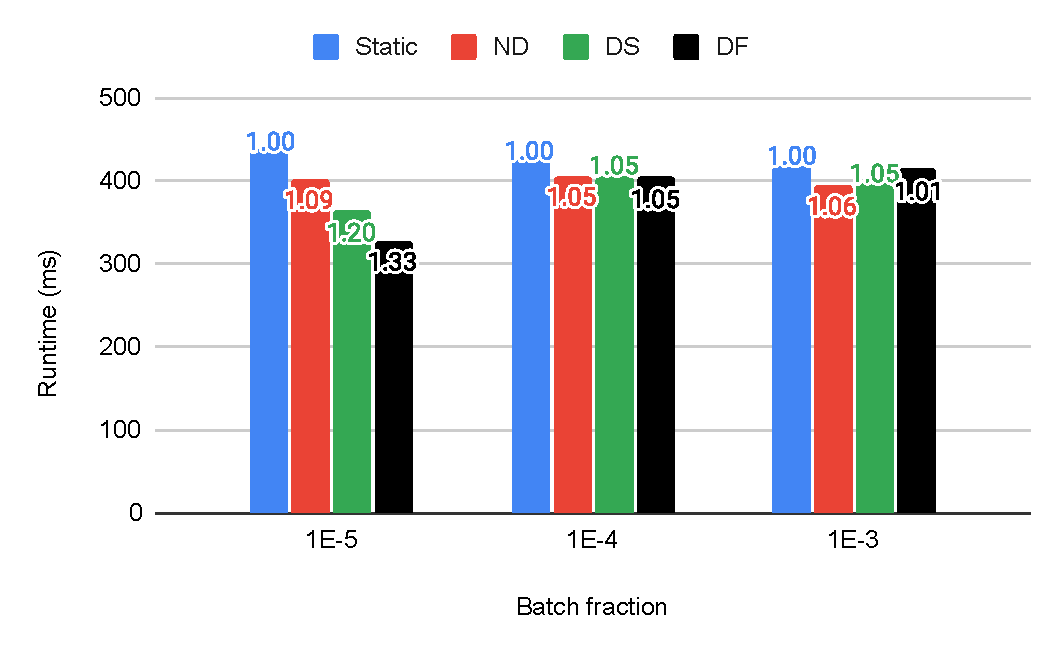
\includegraphics[width=0.48\linewidth]{out/temporal-summary-runtime-overall.pdf}
  }
  \subfigure[Overall Modularity of communities obtained]{
    \label{fig:temporal-summary--modularity-overall}
    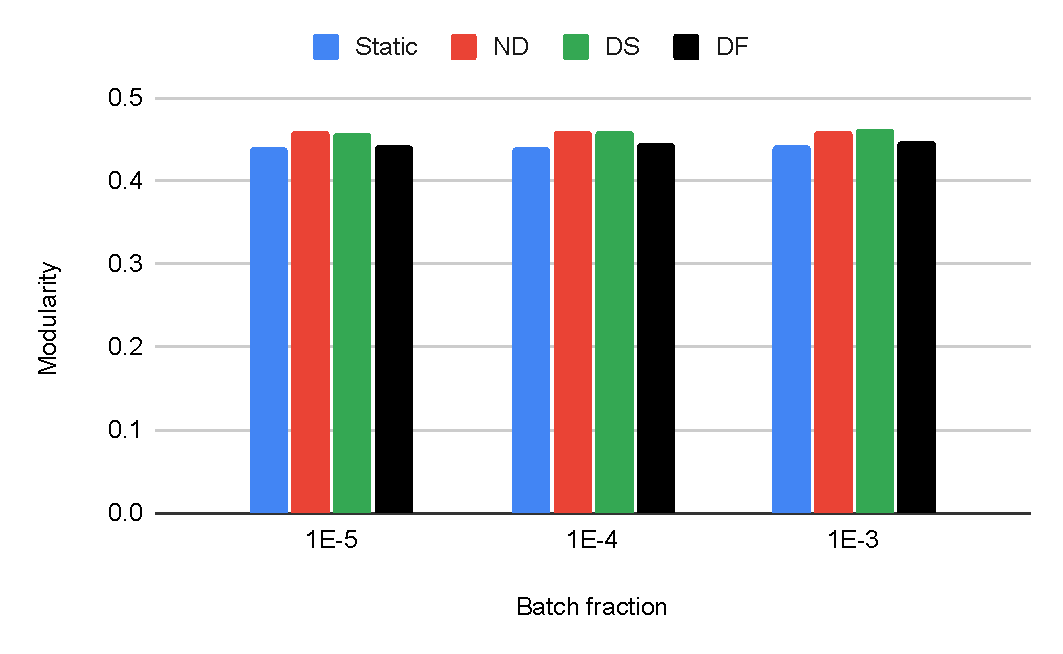
\includegraphics[width=0.48\linewidth]{out/temporal-summary-modularity-overall.pdf}
  } \\[2ex]
  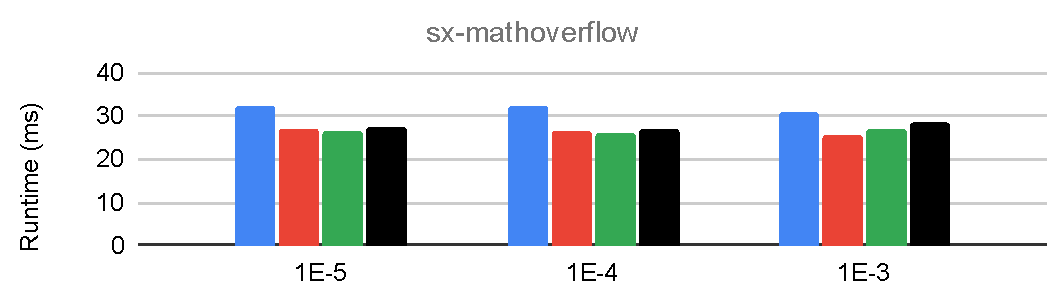
\includegraphics[width=0.48\linewidth]{out/temporal-summary-runtime-sx-mathoverflow.pdf}
  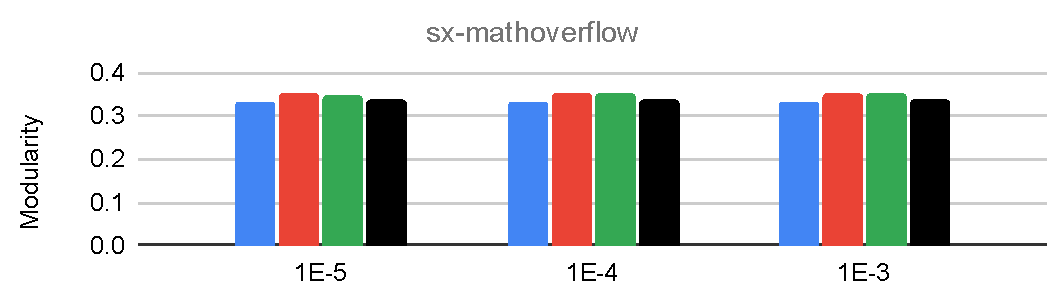
\includegraphics[width=0.48\linewidth]{out/temporal-summary-modularity-sx-mathoverflow.pdf}
  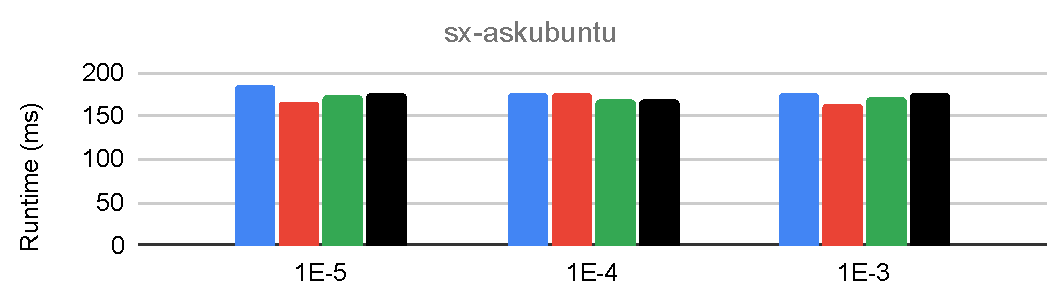
\includegraphics[width=0.48\linewidth]{out/temporal-summary-runtime-sx-askubuntu.pdf}
  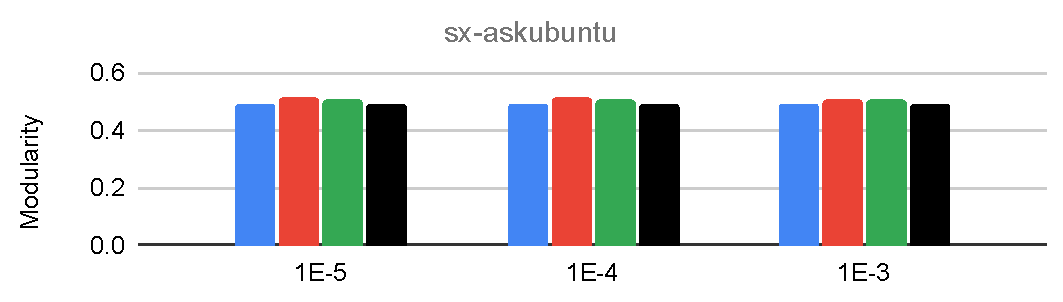
\includegraphics[width=0.48\linewidth]{out/temporal-summary-modularity-sx-askubuntu.pdf}
  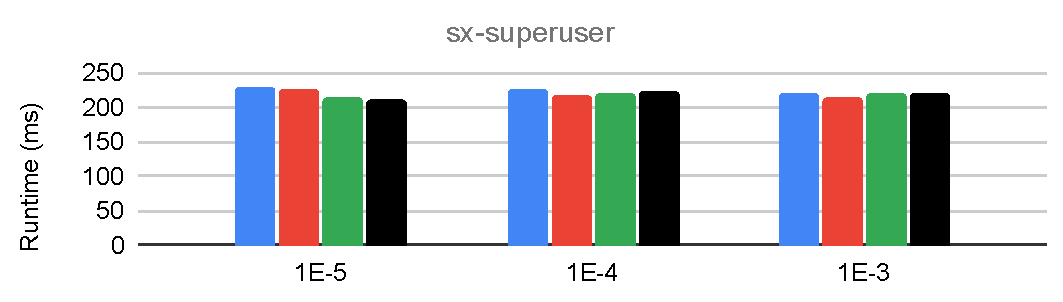
\includegraphics[width=0.48\linewidth]{out/temporal-summary-runtime-sx-superuser.pdf}
  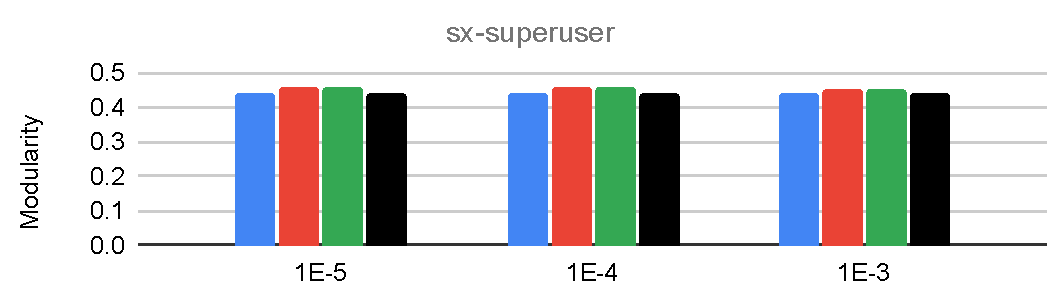
\includegraphics[width=0.48\linewidth]{out/temporal-summary-modularity-sx-superuser.pdf}
  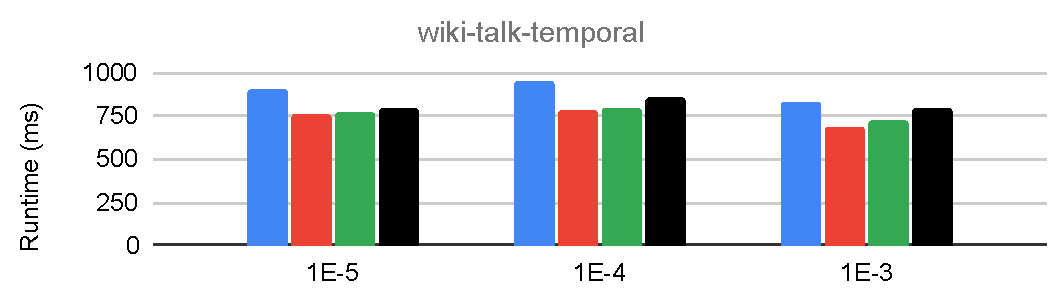
\includegraphics[width=0.48\linewidth]{out/temporal-summary-runtime-wiki-talk-temporal.pdf}
  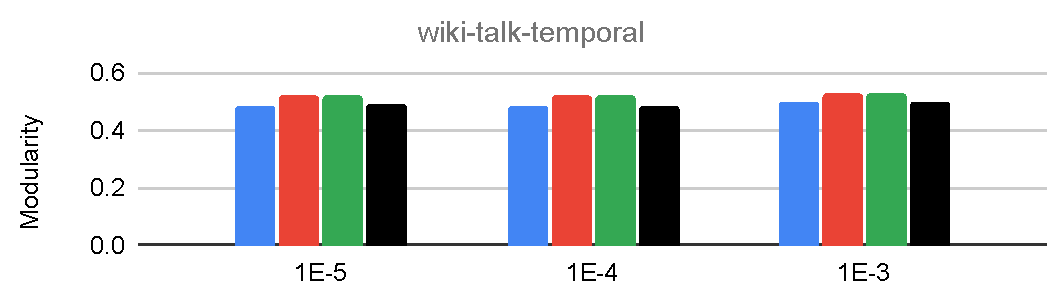
\includegraphics[width=0.48\linewidth]{out/temporal-summary-modularity-wiki-talk-temporal.pdf}
  \subfigure[Runtime on each dynamic graph]{
    \label{fig:temporal-summary--runtime-graph}
    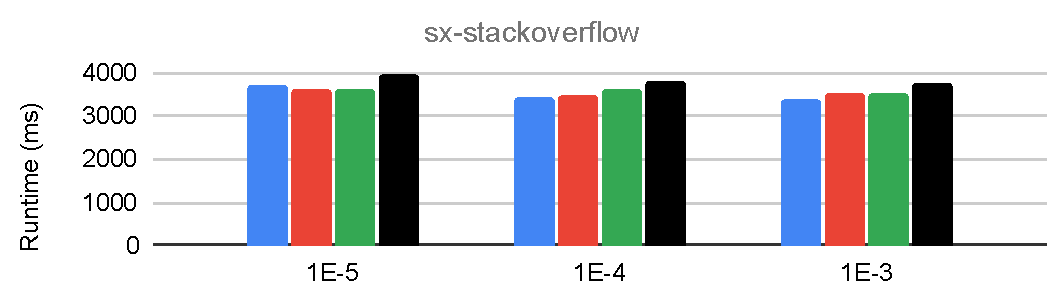
\includegraphics[width=0.48\linewidth]{out/temporal-summary-runtime-sx-stackoverflow.pdf}
  }
  \subfigure[Modularity in communities obtained on each dynamic graph]{
    \label{fig:temporal-summary--modularity-graph}
    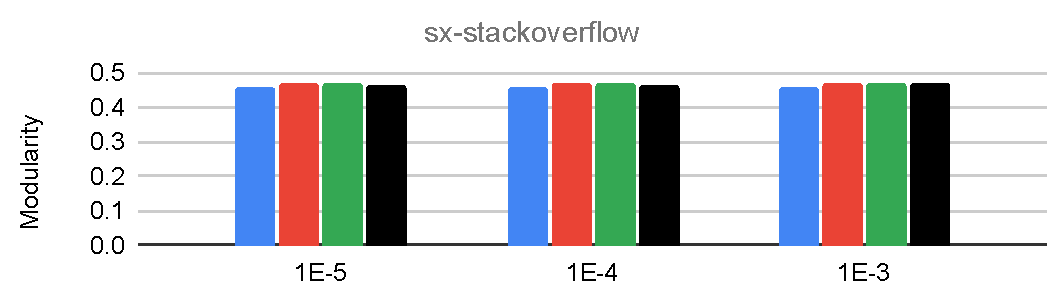
\includegraphics[width=0.48\linewidth]{out/temporal-summary-modularity-sx-stackoverflow.pdf}
  } \\[-2ex]
  \caption{Mean Runtime and Modularity of communities obtained with our multicore implementation of \textit{Static}, \textit{Naive-dynamic (ND)}, \textit{Delta-screening (DS)}, and \textit{Dynamic Frontier (DF)} Leiden on real-world dynamic graphs, with batch updates of size $10^{-5}|E_T|$ to $10^{-3}|E_T|$. Here, (a) and (b) show the overall runtime and modularity across all temporal graphs, while (c) and (d) show the runtime and modularity for each graph. In (a), the speedup of each approach with respect to Static Leiden is labeled.}
  \label{fig:temporal-summary}
\end{figure*}

